\section{Claycode Markers}

In this section we explore an alternative application of Claycodes: rather than encoding data in the code itself, we generate a topology starting from an arbitrary image and use it as the code. Under this design, the actual data is stored elsewhere (e.g. in a cloud application) while the  code itself serves as a key to the data.

\begin{figure}[h]
    \caption{Revised encoding-decoding pipeline.}
    \centering
    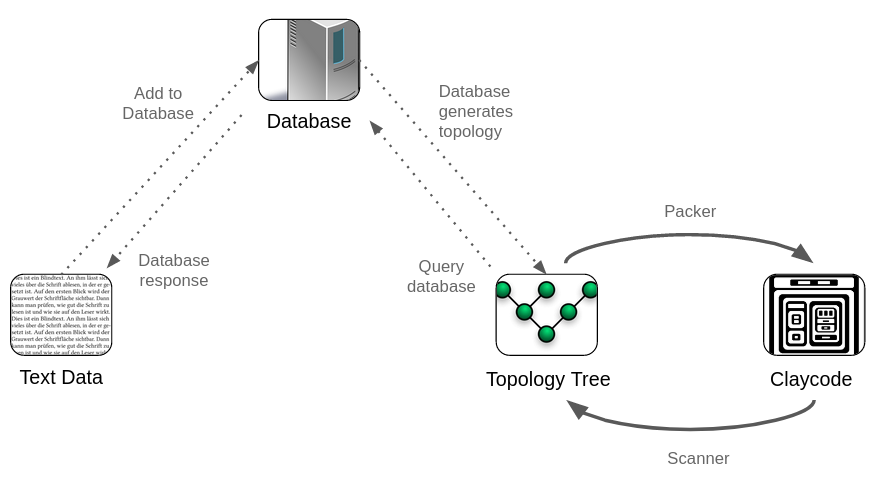
\includegraphics[width=0.45\textwidth]{markers}
\end{figure}

\subsection[artDefined]{Art-Defined Markers}

This approach allows the markers to be stylizable with minimal constraint on the artist.

\subsection[fragments]{Fragmented Markers}

To achieve error correction based on redundancy, we can use a similar approach to instead generate multiple topologies embedded in an arbitrary image. This type of error correction is resistant to certain classes of tampering that QR codes are vulnerable to.
